\chapter{Quantenfeldtheorien zur Beschreibung der Teilchenphysik}
\section{Das Standardmodell der Teilchenphysik}
Das Standardmodell (SM) der Teilchenphysik ist eine Sammlung aus Quantenfeldtheorien und Parametern, die eine Beschreibung der bisher bekannten Elementarteilchen und Wechselwirkungen ermöglicht. Diese Elementarteilchen werden anhand ihrer Quantenzahlen wie Spin, Ladung und Masse klassifiziert.
Es wird zwischen den Fermionen mit einem halbzaligen Spin und den Eichbosonen mit einem ganzzahligen Spin, sowie dem Higgs-Boson mit Spin $0$ unterschieden. Die Fermionen sind die Bausteine der Materie und werden wiederum in Quarks und Leptonen unterschieden. Diese setzen sich jeweils aus drei Generationen, die jeweils aus einem $\text{SU}(2)$ Dublett bestehen, zusammen.\\
Die elementaren Wechselwirkungen werden durch die Eichbosonen vermittelt. Es wird zwischen der durch das Photon $\gamma$ vermittelteten elektromagnetischen Wechselwirkung, der durch die $W^{\pm}$ und $Z^0$ Bosonen vermittelten schwachen Wechselwirkung und der starken Wechselwirkung unterschieden. Letztere wird durch die acht Gluonen $g$ übertragen, die an die Farbladung koppeln.\\
\begin{figure}[H]
  \centering
  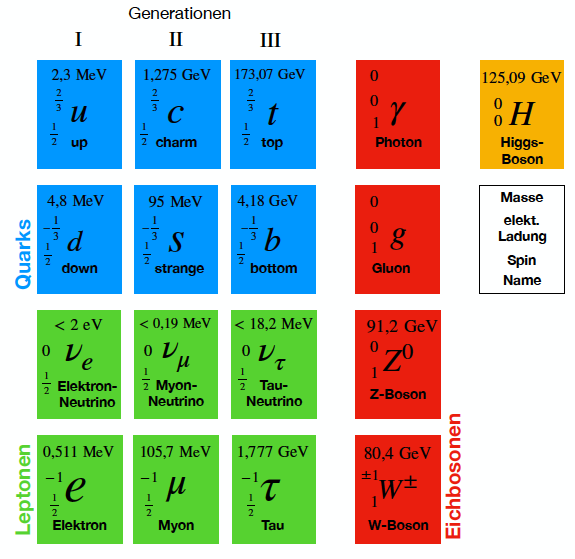
\includegraphics[width=0.6\textwidth]{Plots/SM.png}
  \caption{Schematische Darstellung der Elementarteilchen des SM\cite{Patrignani:2016xqp}.}
\end{figure}
Die Eichsymmetrie $SU(3)_\text{C} \times SU(2)_\text{L} \times U(1)_\text{Y}$ beschreibt diese Wechselwirkungen vor der Symmetriebrechung. Mit dem 2012 entdeckten, skalaren Higgs-Boson \cite{ Aad:2012tfa}\cite{Chatrchyan:2012xdj} kann das heutzutage bekannte SM durch den Lagrangian:
\begin{equation}
  \mathscr{L}_{SM} = - \frac{1}{4}F_{\mu\nu}F^{\mu\nu} + i \overline{\psi}\slashed{D}\psi + \psi_i Y_{ij} \psi_j \Phi + h.c. + |D_{\mu}\Phi|^2 - V(\Phi)
  \label{eqn:LSM}
\end{equation}
beschrieben werden. Der erste Term der Gleichung \eqref{eqn:LSM} beschreibt die kinetische Energie der Eichbosonen $\gamma$, $W^{\pm}$, $Z^0$ und $g$.
Hierbei treten Terme auf, die die Selbstkopplung der Gluonen beschreiben. Der zweite Term beschreibt die kinetische Energie der Fermionen und liefert damit eine Erklärung für die elementaren Wechselwirkungen mit den Eichfeldern.
Durch den Term $\psi_i Y_{ij} \psi_j \Phi + h.c.$ wird die Yukawa Wechselwirkung der Fermionen mit dem Higgsfeld dargestellt.
Dadurch lassen sich die Fermionenmassen und die Kopplung an das Higgs-Boson erklären.
Die kinetische Energie des Higgs-Bosons und damit dessen
Wechselwirkung mit den Eichfeldern wird durch den Term $|D_{\mu}\Phi|^2$ beschrieben. Obwohl Eichbosonen im Allgemeinen masselos sind, tragen das $W^{\pm}$ und $Z^0$ trotzdem eine Masse. Diese wird bei der spontanen Symmetriebrechung der Vereinheitlichung der QED und der schwachen Wechselwirkung $SU(2)_\text{L} \times U(1)_\text{Y}$, die durch den Higgs-Mechanismus verursacht wird, induziert. Der letzte Teil der Gleichung ist das Higgspotential. Dieses beinhaltet den Massenterm des Higgs-Bosons und beschreibt die Selbstkopplung des Higgs.

\section{Effektive Feldtheorie zur Erweiterung des Standardmodells}
Trotz der präzisen Beschreibung der bis heute entdeckten Teilchen und Wechselwirkungen gilt das SM als unvollständig. Es liefert beispielsweise keine Erklärung für die dunkle Materie, die aufgrund der abweichenden Rotationsgeschwindigkeit von Galaxien postuliert wurde \cite{Bertone:2016nfn}. Physikalische Theorien, die Effekte beschreiben, die über das SM hinausgehen, werden allgemein als Physik jenseits des SM (engl. \textit{beyond-the-standard-model}, BSM) bezeichnet. Da bis heute keine neuen Elementarteilchen bei der direkten Suche gemessen wurden, wird angenommen, dass diese zu schwer für die direkte Produktion an den heutigen Beschleunigern sind. Dies lässt vermuten, dass die Energieskala $\symup{\Lambda}$ der BSM-Physik, die des Standardmodells überschreitet. Trotz der aktuell nicht möglichen direkten Produktion könnten die Auswirkungen dieser neuen Teilchen auf andere Prozesse durch neue Effekte beobachtbar sein. Eine geeignete theoretische Beschreibung für diese Phänomene sind effektive Feldtheorien (EFT). Diese sind modellunabhängig und ermöglichen dadurch eine Beschreibung ohne einschränkende Annahmen für neue Wechselwirkungen. Ein sehr bekanntes Beispiel für eine EFT ist Fermis Erklärung des $\beta$-Zerfalls, der sich später mit der schwachen Wechselwirkung erklären ließ\cite{Fermi1934}.\\
Existiert ein neues Teilchen $X$, das leicht genug ist um es direkt zu produzieren, wird die Wechselwirkung mit anderen Teilchen durch den Propagator $\frac{1}{p^2 -m_X^2}$ beschrieben. Wenn dieses Teilchen jedoch zu schwer ist für die direkte Produktion, kann nur die indirekte Auswirkung auf die an der Wechselwirkung beteiligten Teilchen beschrieben werden. In diesem Fall lässt sich der Propagator um $\frac{p^2}{m_X^2}$ entwickeln, sodass er sich zu:
\begin{align}
    \frac{1}{p^2 -m_X^2} = -\frac{1}{m_X^2}\left[ 1 + \frac{p^2}{m_X^2} + \mathcal{O}\left(\frac{p^4}{m_X^4}\right)\right]
\end{align}
ergibt. Dies ermöglicht eine Parametrisierung der Auswirkung neuer Teilchen mit effektiven Operatoren.
Mit diesem Prinzip lassen sich effektive Feldtheorien ebenfalls mit einem Lagrangian beschreiben, der eine Parametrisierung von neuen Teilchen und eventuellen Wechselwirkungen ermöglicht. Die EFT-Operatoren tragen eine höhere Massendimension als die SM-Massendimension vier. Dabei ist zu beachten, dass die Auswirkungen der neuen Operatoren auf messbare Prozesse mit dem Inversen der Energieskala $\frac{1}{\Lambda^{d-4}}$ unterdrückt werden. Somit sinkt mit steigender Ordnung der Einfluss der Operatoren und damit die Wahrscheinlichkeit bei niedrigen Energien die Auswirkungen der entsprechenden Operatoren zu beobachten.\\
Der EFT-Lagrangian ist wie folgt definiert:
\begin{equation}
  \mathscr{L}_{EFT} = \sum_{d,i} \frac{1}{\Lambda^{d-4}} C_i O_i^{(d)}.
\end{equation}
Hierbei beschreiben die $O_i$ neue Operatoren höherer Ordnung und die $C_i$, die sogenannten Wilson-Koeffizienten, die individuellen Stärken dieser. Terme mit Massendimension $5$ entsprechen der Einführung von Majorana Massentermen. Diese sind jedoch für die Physik am Large Hadron Collider (LHC) uninteressant, da kein eichinvarianter Operator definiert werden kann, bei dem SM Quarks beteiligt sind. Somit können im Bereich der Top-Quark-Physik keine Effekte von Operatoren mit Massendimension fünf gemessen werden. Bei der Massendimension sechs ergeben sich hingegen insgesamt $59$ effektive Operatoren \cite{Grzadkowski:2010es}, von denen $15$\cite{Zhang:2014rja} an das
Feld des Top-Quarks koppeln.\\
Für die Operatoren mit der Massendimension sechs lässt sich ein Lagrangian durch:
\begin{equation}
  \mathscr{L}_{EFT, 6} = \mathscr{L}_{SM} + \mathscr{L}_{dim6} = \mathscr{L}_{SM} + \frac{1}{\Lambda^{2}} C_i O_i^{(6)}
\end{equation}
formulieren. Da der Lagrangian $\mathscr{L}_{EFT, 6}$ ebenfalls die Eichsymmetrie des SM erfüllen muss, geht er im Grenzfall in das Standardmodell über, sodass die Wilson-Koeffizienten in diesem Fall alle gleich 0 sind.

\section{Das Top Quark im Zusammenhang mit effektiver Feldtheorie}
\label{top}
Das Top Quark trägt Spin $\frac{\hbar}{2}$ und neben der elektrischen Ladung von $\frac{2}{3}$ der
Elementarladung $e$ auch eine Farbladung. Es nimmt wie alle Quarks an den drei fundamentalen Wechselwirkungen
teil. Durch seine hohe Masse $m_t = \SI{173.34(76)}{\giga\electronvolt}$~\cite{ATLAS:2014wva}, der höchsten eines
Elementarteilchens im SM, besitzt es nur eine sehr kurze Lebensdauer. Deshalb hadronisiert das
$t$-Quark nicht wie andere Quarks durch die starke Wechselwirkung, sondern zerfällt hauptsächlich über die schwache Wechselwirkung in ein $W$-Boson und ein $b$-Quark, wie in der CKM-Matrix an $|V_{tb}|^2 \approx 1$ zu erkennen ist.
Dieser Zerfall hat eine deutliche Signatur, die es ermöglicht eine sehr genaue Bestimmung der Quantenzahlen des Top-Quarks durchzuführen, sodass eine hohe Sensitivität in Bezug auf mögliche Abweichungen durch BSM-Physik erreicht wird.
Der Grundgedanke bei der Suche nach neuen physikalischen Effekten ist, dass neue Teilchen auf Grund ihrer hohen Masse besonders stark an das Higgs-Boson koppeln. Da das $t$-Quark das einzige SM-Fermion ist mit einer Yukawa-Kopplung von ungefähr $1$, wird davon ausgegangen, dass es ebenfalls besonders stark an die neuen Teilchen koppelt. Dies motiviert eine genaue Untersuchung des Top-Sektors in Bezug auf BSM-Physik.\\
Ein Prozess bei dem möglicherweise BSM-Physik-Effekte beitragen, ist die Abstrahlung eines Photons an einem $t$-Quark. Dies kann mit einem effektiven Vertex, wie in Abbildung~\ref{fig:eftVertex} dargestellt, beschrieben werden. Die Betrachtung dieses Vertex ist dadurch motiviert, dass er ebenfalls in einem Schleifenprozess in der $b$-Physik, wie in Abbildung~\ref{fig:bsa} dargestellt, vorkommt. Dort wurde bereits nach Auswirkungen von BSM-Physik gesucht. Daher ist es interessant zu untersuchen, ob die beteiligten Wilson-Koeffizienten des Vertex in der Top-Physik zu den gleichen Eingrenzungen führen.\\
Grundlage dieser Arbeit ist der $t\bar{t}\gamma$ Produktionswirkungsquerschnitt, der zum Beispiel in Prozessen wie in Abbildung~\ref{fig:tta} verdeutlicht, vorkommt. Hierbei kommt es zu Wechselwirkungen, die durch die drei BSM-Operatoren $O_{tB}, O_{tW}$ und $O_{tG}$ beschrieben werden können\cite{Bylund:2016phk}.
\begin{figure}
  \centering
  \begin{tikzpicture}
    \begin{feynman}
      \vertex (q1) {\(t\)};
      \vertex [right=1.5cm of q1, blob] (q2) {};
      \vertex [below right=1.5cm of q2] (q3) {\(\gamma\)};
      \vertex [above right=1.5cm of q2] (q4) {\(t\)};

      \diagram* {
        (q1) -- [fermion] (q2) -- [fermion] (q4),
        (q2) -- [boson] (q3),
      };
    \end{feynman}
  \end{tikzpicture}
  \caption{Darstellung des effektiven Vertex bei der Abstrahlung eines Photons $\gamma$ am $t$-Quark.}
  \label{fig:eftVertex}
\end{figure}
Dabei wird $O_{tG}$ betrachtet, weil das $t$-Quark aus Gluonfusion entsteht und $O_{tB}$ und $O_{tW}$ wegen der Photonabstrahlung.
\begin{align}
   O_{tW} &= y_t g_w \left(\bar{Q}\sigma^{\mu\nu}\tau^{I} t \right) \tilde{\varphi} W^{I}_{\mu\nu}\\
   O_{tB} &= y_t g_Y \left(\bar{Q}\sigma^{\mu\nu} t \right) \tilde{\varphi} B_{\mu\nu}\\
   O_{tG} &= y_t g_s \left(\bar{Q}\sigma^{\mu\nu}T^A t\right)\tilde{\varphi}~ G^{A}_{\mu\nu}
\end{align}
Hierbei steht $Q$ für das linkshändige Quarkdublett der dritten Generation, $\varphi$ für das Higgsfeld und $g_w$, $g_Y$ und $g_s$ sind die SM Eichkopplungskonstanten. Die Yukawa Kopplung des Top-Quarks wird mit $Y_t = \frac{\sqrt{2}m_t}{v}$ beschrieben, bei der $v = \SI{246}{\giga\electronvolt}$ der Higgsvakuumserwatungswert ist.\\
Dies motiviert die Wilson-Koeffizienten dieser Operatoren hier näher zu untersuchen. Wenn ein Vergleich dieser Operatoren mit denen, die bei dem Prozess \ref{fig:bsa} beteiligt sind, angestrebt wird, muss beachtet werden, dass sich die Benennung unterscheidet und die Bestimmung auf unterschiedlichen Energieskalen erfolgt.

\begin{figure}
  %\centering
    \begin{subfigure}[b]{0.45\textwidth}
      \centering
      \begin{tikzpicture}
        \begin{feynman}
            \vertex (a) {\(g\)};
            \vertex [below=1.5cm of a] (b) {\(g\)};
            \vertex [below right=1cm of a] (a1);
            \vertex [right=1cm of a1] (a2);
            \vertex [above right=1cm of a2] (a4);
            \vertex [above left= 1cm of a4] (a5) {\(\gamma\)};
            \vertex [above right=0.5cm of a4] (a3);
            \vertex [above right=1cm of a3] (c);
            \vertex [above right=0.5cm of c] (c1) {\(q_{1}\)};
            \vertex [below right=0.5cm of c] (c2) {\(\bar{q}_2\)};
            \vertex [below=0.5cm of c2] (d) {\(\bar{b}\)};
            \vertex [below right=0.5cm of a2] (b1);
            \vertex [below right=1cm of b1] (b2);
            \vertex [above right=1cm of b2] (b3);
            \vertex [above right=0.5cm of b3] (d1) {\(l^{-}\)};
            \vertex [below right=0.5cm of b3] (d2) {\(\bar{\nu}_l\)};
            \vertex [below=0.5cm of d2] (d3) {\(b\)};
            \diagram* {
              (a) -- [gluon] (a1),
              (b) -- [gluon] (a1) -- [gluon] (a2),
              (a2) -- [anti fermion, edge label=\(\overline t\)] (a3) -- [anti fermion] (d),
              (a3) -- [boson, edge label=\(W^{-}\)] (c) -- [fermion] (c1),
              (c) -- [anti fermion] (c2),
              (a2) -- [fermion, edge label'=\(t\)] (b2),
              (b2) -- [boson, edge label=\(W^{+}\)] (b3) -- [fermion] (d1),
              (b3) -- [anti fermion] (d2),
              (b2) -- [fermion] (d3),
              (a4) -- [boson] (a5),
            };
        \end{feynman}
      \end{tikzpicture}
      \subcaption{Zerfall eines $t$-Quarks in ein $W$-Boson und ein $b$-Quark unter Abstrahlung eines Photons~$\gamma$.}
      \label{fig:tta}
    \end{subfigure}
    \hfill
    \begin{subfigure}[b]{0.45\textwidth}
      \centering
      \begin{tikzpicture}
        \begin{feynman}
          \vertex (a1) {\(b\)};
          \vertex[right=1.5cm of a1] (a2);
          \vertex[right=1cm of a2] (a3);
          \vertex[below=1cm of a3] (c2) {\(\gamma\)};
          \vertex[right=1cm of a3] (a4);
          \vertex[right=1.5cm of a4] (a5) {\(s\)};
          \diagram* {
          (a1) -- [fermion](a2),
          (a2) -- [fermion, edge label'=\(t\)] (a3),
          (a3) -- [boson] (c2);
          (a3) -- [fermion, edge label'=\(t\)] (a4),
          (a4) -- [fermion] (a5),
          (a4) -- [boson, out=90, in=90, looseness=2, edge label'=\(W^{-}\)] (a2)
          };
        \end{feynman}
      \end{tikzpicture}
      \subcaption{Zerfall eines $b$-Quarks in ein $s$-Quark unter Abstrahlung eines Photons~$\gamma$ im Loop.}
      \label{fig:bsa}
    \end{subfigure}
  \caption{Prozesse aus der Top-Quark- und der Bottom-Quark-Physik bei denen der effektive Vertex $t\bar{t}\gamma$ beteiligt ist.}
\label{fig:feynman}
\end{figure}
